\section{Convolutional neural networks}

The central method used in this project is a deep learning algorithm called convolutional neural networks (\abbrCNN for short). A \abbrCNN architecture can successfully capture the spatial dependencies in an image through convolutional filtering operations with kernels of learnable weights and biases.

\begin{figure}[H]
	\centering
	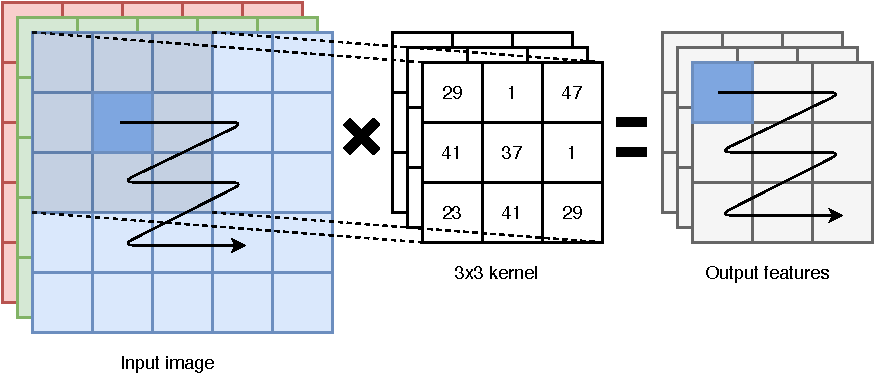
\includegraphics[width=0.9\textwidth]{conv}
	\caption{Convolutional filtering operation with a 3 channel RGB image and 3x3 kernel}
	\label{fig:conv}
\end{figure}

In Figure \ref{fig:conv} a convolutional filtering operation over an image is illustrated. The matrix kernel is moved in a row by row pattern and is multiplied by a patch of the image to get a value for the output cell.

In order to form a deep neural network multiple filtering operations are chained sequentially with nonlinear activation functions between them. A deep neural network usually consists of many such layers of filtering operations and activation functions. This concept is illustrated in Figure \ref{fig:deep}.

\begin{figure}[H]
	\centering
	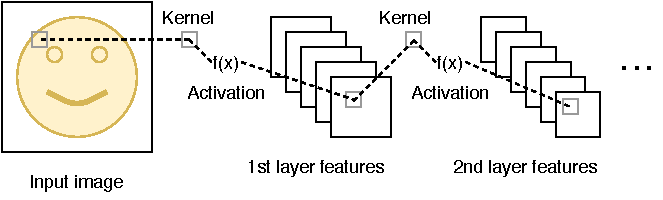
\includegraphics[width=0.8\textwidth]{deep}
	\caption{Multiple layers chained with each other to form a deep network}.
	\label{fig:deep}
\end{figure}

The activation functions need to be differentiable because the derivatives are used in the learning process. Some common nonlinear activation functions are shown in Figure \ref{fig:activation}.

\begin{figure}[H]
	\centering
	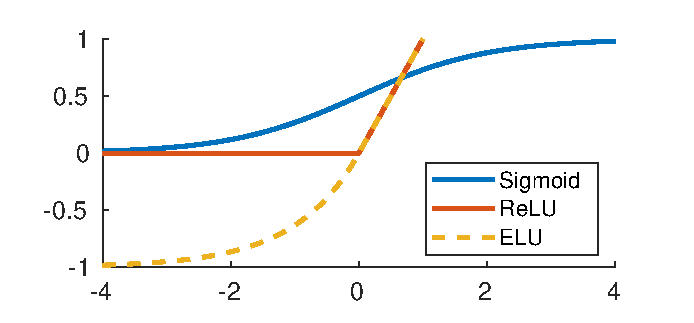
\includegraphics[width=0.6\textwidth]{activation}
	\caption{A few common nonlinear activation functions.}
	\label{fig:activation}
\end{figure}

The features in the deep neural networks are used to formulate a loss function. The loss defines an objective that we want the network to learn. This means that the process of learning becomes a task of updating the filter kernels in such a way that the loss function is minimized. If the loss function is decreasing during the training process it means that the network is learning. It is crucial that the loss function describes the problem accurately, otherwise the network will not learn the correct behavior. The weights in the network are updated using a method called back propagation. The algorithm computes the gradient of the loss function with respect to the weights in the network for a single input example from the training data using the derivative chain rule, which can be done very efficiently. Updating the weights to minimize the loss function can then be done using gradient decent. As the network is fed with more input examples from the training data, the network slowly learns the correct weights that minimizes the loss function as desired.


